\documentclass{article}
\usepackage[utf8]{inputenc}
\usepackage{fancyhdr}
\usepackage{graphicx}
\usepackage{geometry}
\usepackage{float}

% ---- Commands ------- %
\newcommand{\documentNumber}[1]{
    \LARGE  \textbf{ Kravspecifikation }
    \\
    \medskip
}
\newcommand{\documentVersion}[1]{
    \medskip
}
\newcommand{\documentTitle}[1]{
    \centerline{\rule{13cm}{0.4pt}}
    \bigskip \bigskip
    \LARGE \textbf{Projekt IDA3} \\
    \bigskip
    \LARGE {#1} \\
    \bigskip \bigskip
    \centerline{\rule{13cm}{0.4pt}}
}

\newcommand{\documentDate}[1]{
    \date {#1} 
}


\renewcommand{\arraystretch}{1.7}  % Vertical padding for tables

\renewcommand{\contentsname}{Innehållsförtäckning}

% --- Header & Footer ---- %
\pagestyle{fancy}
\lhead{\leftmark}
\rhead{}
\rfoot{\thepage}
\cfoot{}
\lfoot{}


% ------------------------------------------------ #

% ----- FILL THIS ----- %
\title {
    \documentNumber {01}    

    % Full name - SHORTNAME
    \documentTitle {Helsingborg Event and Convention Bureau}
    
    % Format: YYYY-MM-DD
    \documentDate {2021-08-20}
    \documentVersion Vv 0.2
    
    \author{Anna Bergvall - Oscar Blixt - Pontus Persson - Filip Sjövall - David Vilppu - Sahab Zafar}
}

\begin{document}
\addtocontents{toc}{\protect\setcounter{tocdepth}{2}}
\maketitle

\thispagestyle{empty}



\newpage

\tableofcontents


\newpage

\section{Dokument Historia}
\begin{tabular}{ l | l | l }
    Version & Date & Description \\
    \hline
    0.1 & 2021-10-06 & Dokumentet skapat. \\
    0.2 & 2021-11-05 & Första utkast\\
    
\end{tabular}

\section{Introduktion}
    Detta dokument innehåller kraven för ett rapporteringssystem, härefter kallat "systemet", utvecklat på beställning av Helsingborg Convention and Event Bureau. Systemet är ett frågeformulär vars syfte är att få Helsingborg miljöcertifierat av GDSM (Global Destination Sustainability Movement. Huvudfunktionaliteten är att HASAB ska kunna sammanställa den data som tillkommit till följd av svar på formuläret från näringslivet. Systemet ska kunna interagera med databas, server och klient.
    

\section{Bakgrund och mål}

    \subsection{Mål}
      Syftet med projektet är att få Helsingborg stad att bli miljöcertifierad genom att utveckla ett webbaserat frågeformulär som är snabbt och enkelt för användaren att svara på. När datan väl samlats in är det vår uppgift att ta fram en sammanställning som matchar GDSM:s målformat.
        
    \subsection{Viktiga aktörer}
    Systemet kan användas av följande intressenter:
    \begin{itemize}
        \item \textbf{Slutanvändare:} Slutanvändaren kommer interagera med systemet genom att logga in och svara på de frågor som är relevant för dennes bransch.
        \item \textbf{HASAB:} HASAB ska tilldelas rollen administratör och således ha tillgång till en administrationssida där de kan ta bort, lägga till och redigera frågor och användare.
     \end{itemize}
    
    \section{Terminologi}
    \begin{itemize}
        \item \textbf{HASAB:} Förkortning av Helsingborg Arena och Scen AB vilket är företaget som ska utnyttja systemet.
        \item \textbf{Frågeformulär:} Ett webbaserat system som innehåller frågor med flervalsalternativ samt statistikföring över svaren.
        \item \textbf{Administratör:} Administratören har tillgång till systemets alla funktioner.
        \item \textbf{Slutanvändare:}  De personer som svarar på frågeformuläret, vilka främst arbetar inom besöksnäringen i Helsingborgs stad. 
        \item\textbf{Stabila krav:}  Stabila krav är krav som inte är ändringbenägna - de baseras på funktioner som är grundläggande för att systemet ska möta beställarens behov.
        \item \textbf{Ändringbenägna krav:}  Krav som är listade här kan förändras eller tas bort.
        \item \textbf{Uteslutna krav:}  Krav som är listade här är inte längre aktuella.
    \end{itemize}
    
    \section{Hemsidans design}
    
    \subsection*{Stabila krav}
     
    \subsection*{Ändringsbenägna krav}
     \subsubsection*{R1}
    Systemet ska ha ett utseende likt bilden nedan.
    
    \begin{figure}[h!]
    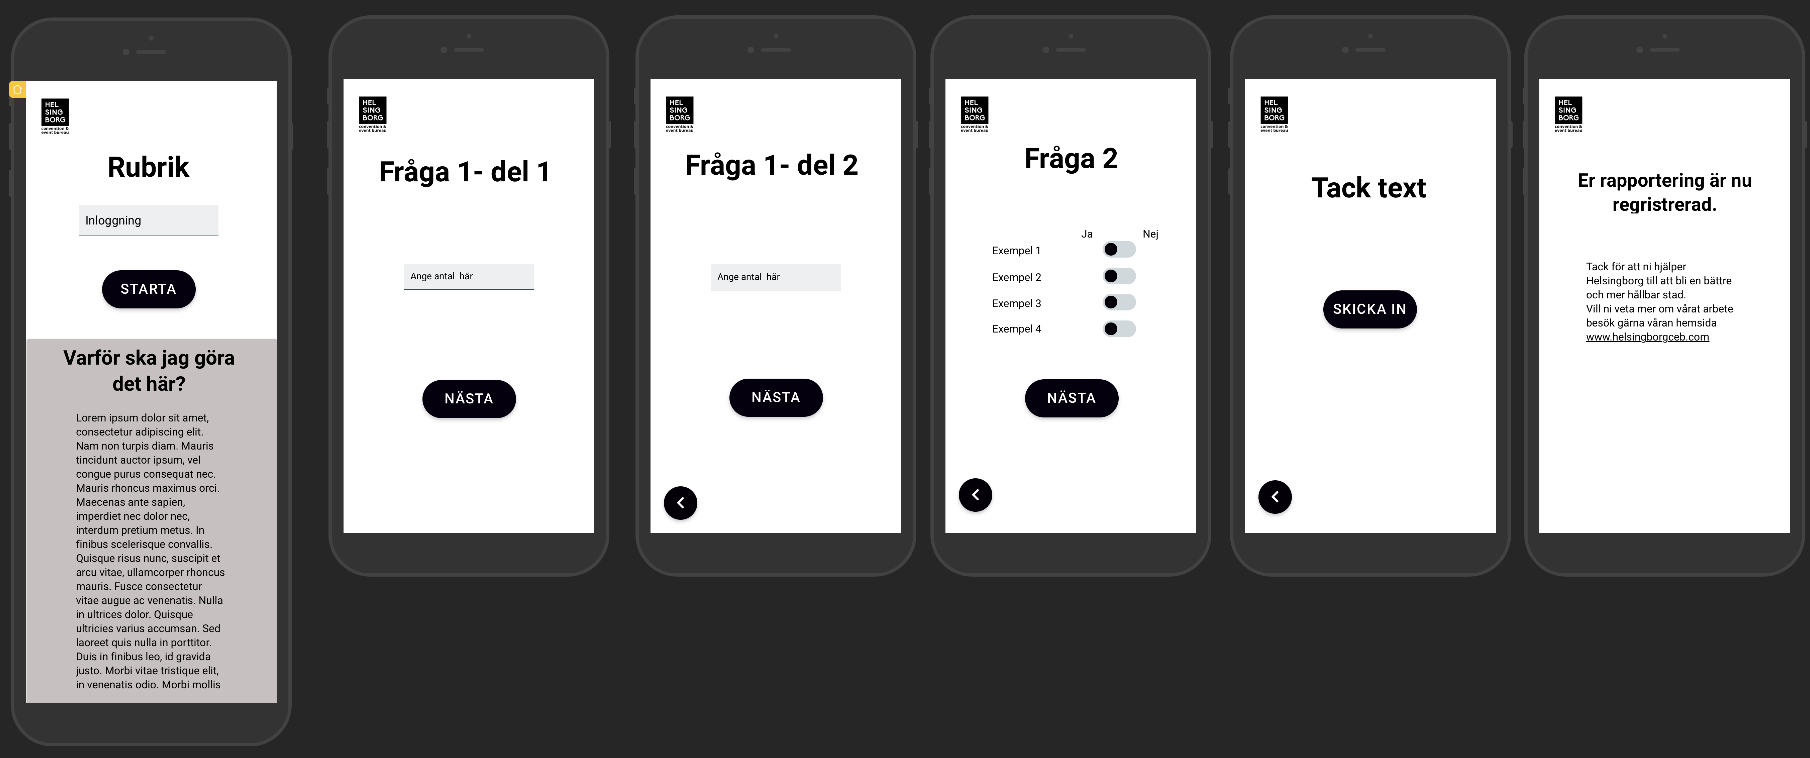
\includegraphics[width=150mm]{prototyp.png}
     \caption{prototyp}
    \end{figure}
    \subsection*{Uteslutna krav}
    
    \section{Hemsidans funktion}
    
    \subsection*{Stabila krav}
    \subsection*{Ändringsbenägna krav}
    
      \subsubsection*{R2}
    Följande scenario ska stödjas av systemet.
        \\
       \indent \textbf{Scenario:} Slutanvändaren navigerar till hemsidan via mail.
        \\
       \indent \textbf{Förutsättningar:} Slutanvändaren har mått ett mail med en länk till hemsidan.
            \begin{enumerate}
                \item Slutanvändaren klickar på länken till formuläret som finns i mejlet.
                \item Slutanvändaren möts av formulärets startsida.
            \end{enumerate}
            
        \subsubsection*{R3}
    Följande scenario ska stödjas av systemet.
        \\
       \indent \textbf{Scenario:} Slutanvändaren ska registrera sig på hemsidan för att få fortsätta rapportering.
        \\
       \indent \textbf{Förutsättningar:} Slutanvändaren har fått en engångskod i samma mail som länken samt att slutanvändaren befinner sig på startsidan.
            \begin{enumerate}
               \item Slutavändaren skriver in koden som finns i mejlet.
               \item Slutanvändaren trycker på knappen "Gå vidare".
                \item  Användaren är nu registrerad och möts av en ny sida med första frågan.
            \end{enumerate}
   
        \subsubsection*{R4}
    Följande scenario ska stödjas av systemet.
        \\
       \indent \textbf{Scenario:} Slutanvändaren ska skicka in slutgiltig rapportering.
        \\
       \indent \textbf{Förutsättningar:} Slutanvändaren har svarat på samtliga frågor och befinner sig på sidan med den sista frågan.
            \begin{enumerate}
                \item Slutanvändaren klickar på knappen "Slutför formulär".
                \item Slutanvändaren möts av en sidan med tack text enligt krav 5.2.1.
                \item Slutanvändaren trycker på knappen "Skicka in formulär".
                \item   Slutanvändaren möts av en bekräftelsesida som bekräftar att formuläret är inskickat.
            \end{enumerate}

\subsubsection*{Krav från scrumboard}
Följande mapning gäller för de krav som finns på projektets scrumboard,\\ d.v.s https://majken.atlassian.net/jira/software/projects/SF/boards/1.\\
När ett krav ska refereras till använd denna graf.\\
$$SR1\rightarrow SF-1$$
$$SR2\rightarrow SF-5$$
$$SR3\rightarrow SF-6$$
$$SR4\rightarrow SF-7$$
$$SR5\rightarrow SF-9$$
$$SR6\rightarrow SF-12$$
$$SR7\rightarrow SF-22$$
$$SR8\rightarrow SF-13$$
$$SR9\rightarrow SF-14$$
$$SR10\rightarrow SF-16$$
$$SR11\rightarrow SF-17$$
$$SR12\rightarrow SF-18$$
$$SR13\rightarrow SF-21$$
$$SR14\rightarrow SF-25$$
$$SR15\rightarrow SF-64$$
$$SR16\rightarrow SF-65$$
$$SR17\rightarrow SF-73$$
$$SR18\rightarrow SF-74$$

    \subsection*{Uteslutna krav}
    
    \newpage
     \section{Hemsidans hantering av data}
    
    \subsection*{Stabila krav}
    \subsubsection*{R5}
    Systemet ska ha fungera enligt diagramet nedan.
    
    \begin{figure}[h!]
    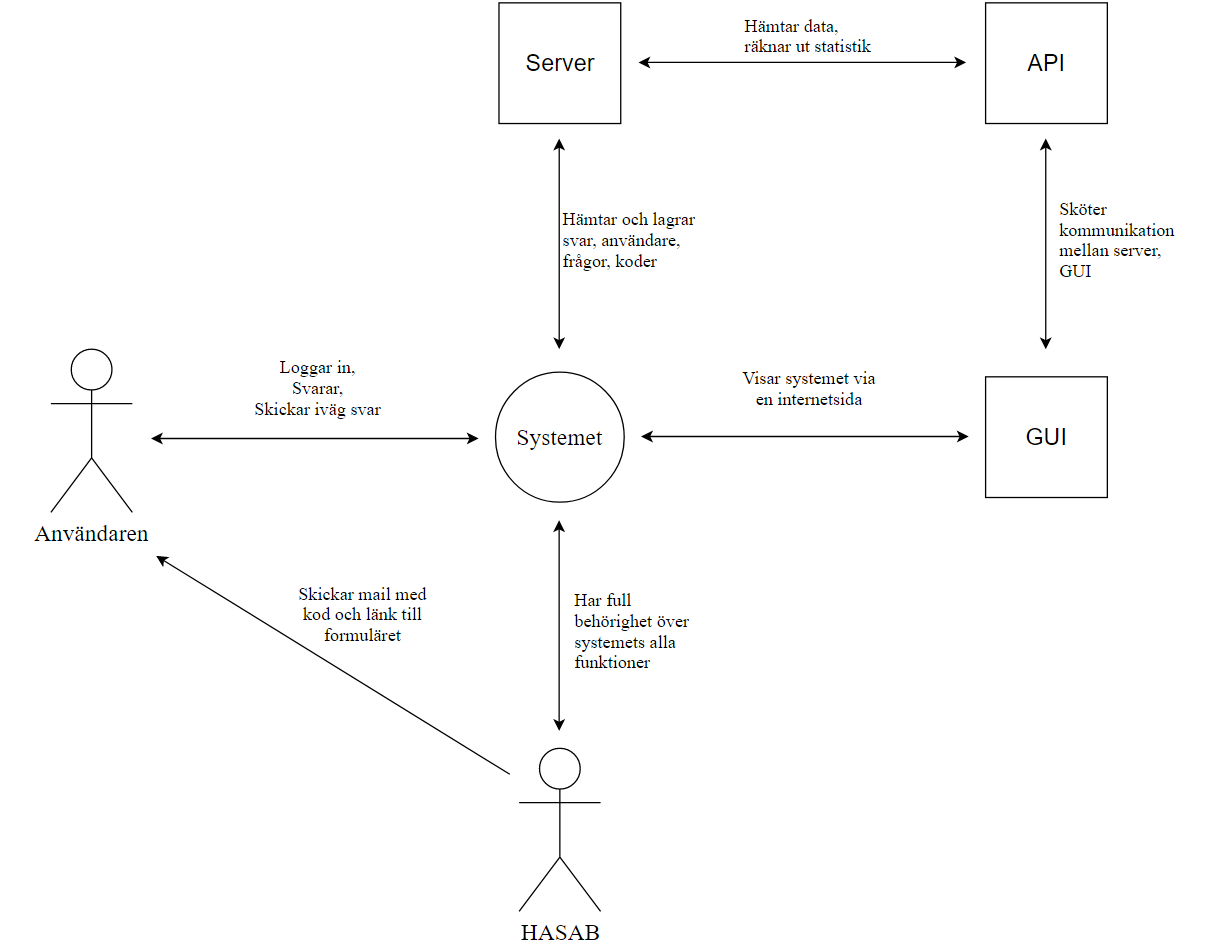
\includegraphics[width=150mm]{Kontextdiagram.png}
    \caption{Kontext-diagram}
    \end{figure}
    
    \newpage
    \subsubsection*{R6}
    Systemt ska hantera data enligt diagrammet nedan.
       \begin{figure}[h!]
    
    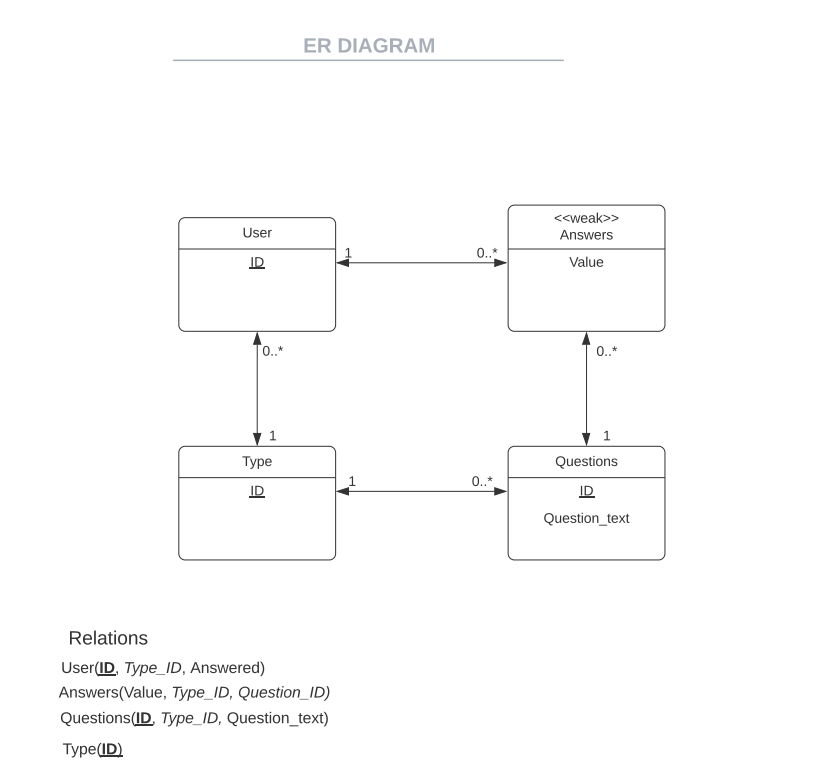
\includegraphics[width=150mm]{ERDIAGRAM.png}
    \caption{ER-Diagram}
    \end{figure}
    
    \newpage
    \subsection*{Ändringsbenägna krav}
    \subsection*{Uteslutna krav}
    
  
   
    \section{Kvalitetskrav}
    \subsection*{Stabila krav}
  
     \subsection*{Ändringsbenägna krav}
     
     \subsubsection*{R7}
    Systemet ska ha en svarstid på max *Open Metric* sekunder.
    
    \subsubsection*{R8}
    Rapportering i systemet ska endast kunna göras av en användare som har fått tillgång till hemsidan via mail eller av admin.
    
     \subsubsection*{R9}
    *Open Metric* användare ska kunna besvara enkäten inom *Open Metric* minuter.
    
    \subsubsection*{R10}
    *Open Metric* användare ska anse att enkäten var lätt att svara på.
    
    \subsection*{Uteslutna krav}
\bibliographystyle{alpha}


\end{document}